This examples is implemented for validating that the ROMC
implementation works accurately in a multidimensional parameter
space.

\subsubsection*{Problem Definition}

The equation that model the inference problem are presented below.

\begin{gather}
  p(\thetab) = p(\theta_1)p(\theta_2)
  = \mathcal{U}(\theta_1; -2.5, 2.5) \mathcal{U}(\theta_2; -2.5, 2.5)\\
  p(\yb|\thetab) = \mathcal{N}(\yb;\thetab, \mathcal{I})\\
  p(\thetab|\yb) = \frac{1}{Z}p(\thetab)p(\yb|\thetab)\\
  Z = \int_{\thetab} p(\thetab)p(\yb|\thetab) d\thetab
\end{gather}

Computing the unnormalised posterior is straightforward using the
equation and approximating the partition $Z$ is feasible with using
the Riemann's approximation. Hence, computing the ground-truth
posterior is computationally feasible. Setting the observation to
$\data=(-0.5,0.5)$, the posterior distribution is illustrated in
figure \ref{fig:ex2_4}. In table \ref{tab:ex2}, we present the
ground-truth statistics i.e.\ $\mu, \sigma$ of the marginal
posterior distributions.

\subsubsection*{Performing the inference}

We perform the inference using the following hyperparameters
$n_1=500, n_2=30, \epsilon=0.4$. This set-up leads to a total of
$15000$ samples. As observed in the histogram of distances
\ref{fig:ex2_1}, in the gradient-based approach, all optimisation
problems reach an almost zero distance end point; hence all optimal
points are accepted. At the Bayesian optimisation scheme, the grand
majority of the optimisation procedures has the behaviour; there are
only 4 optimal distance above the limit. In figure \ref{fig:ex2_2},
the acceptance area of a specific optimisation problem is
demonstrated. We observe that both optimisation schemes lead to a
similar bounding box construction. This specific example is quite
representative of the rest optimisation problems; due to the
simplicity of the optimisation process, in most cases the optimal
points are similar and the surrogate model represents accurately the
local region. Hence, similar proposal regions are obtained using both
optimisation alternatives.

The histograms of the marginal distributions, based on the weighted
samples, is presented in figure \ref{fig:ex2_3}. In the same figure,
we can also plot the ground-truth distribution with the red dotted
line. We observe that the weighted samples, follow quite accurately
the ground-truth distribution. This is also confirmed by the
statistics provided in table \ref{tab:ex2}; the sample mean $\mu$ and
standard deviation $\sigma$ are similar to the ground-truth for both
parameters $\theta_1$ and $\theta_2$. We also observe that they are
almost the same between the two optimisation schemes.

Finally, the ground-truth and the approximate posteriors are presented
in figure \ref{fig:ex2_4}. We also confirm that the approximations are
close to the ground truth posteriors. As a notice, we can observe that
the approximate posteriors ... a diamond shape in the mode of the
posterior; this happens due to the approximation of a circular
gaussian-shape posterior with a sum of square boxes.  The divergence
between the ground-truth distribution and the approximate ones is
$0.077$, using the Jensen-Shannon distance.

In this experiment we observed that the implementation fulfilled the
theoretical expectations for the ROMC inference method.

\begin{center} \label{tab:ex2}
\begin{tabular}{ c|c|c|c|c }
\hline
& $\mu_{\theta_1}$ & $\sigma_{\theta_1}$ & $\mu_{\theta_2}$ & $\sigma_{\theta_2}$ \\
\hline \hline
Ground-truth & -0.45 & 0.935 & 0.45 & 0.935 \\
\hline
ROMC (gradient-based) & -0.482 & 0.976 & 0.522 & 0.945 \\
\hline
ROMC (Bayesian optimisation) & -0.481 & 0.976 & 0.518 & 0.947 \\
\hline
\end{tabular}
\end{center}


\begin{figure}[h]
    \begin{center}
      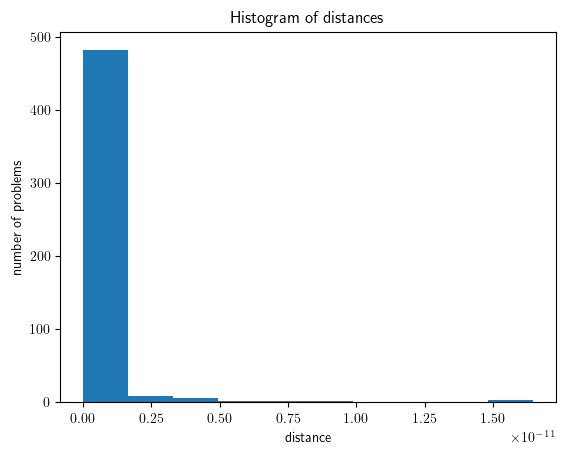
\includegraphics[width=0.48\textwidth]{./Thesis/images/chapter4/ex2D_distance_hist.png}
      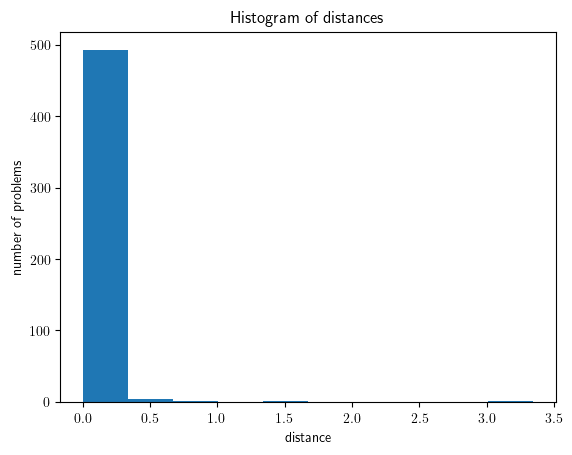
\includegraphics[width=0.48\textwidth]{./Thesis/images/chapter4/ex2D_distance_hist_bo.png}
    \end{center}
    \caption{Histogram of distances $d_{i, i \in {1, \ldots,
          n_1}}^*$. The left graph corresponds to the gradient-based
      approach and the right one to the Bayesian optimisation
      approach.}
  \label{fig:ex2_1}
\end{figure}


\begin{figure}[h]
    \begin{center}
      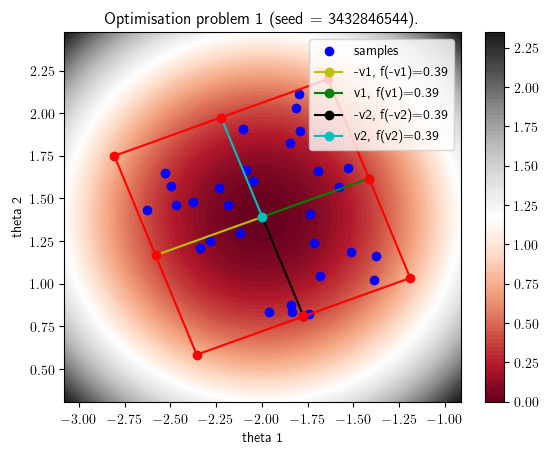
\includegraphics[width=0.48\textwidth]{./Thesis/images/chapter4/ex2D_region_1.png}
      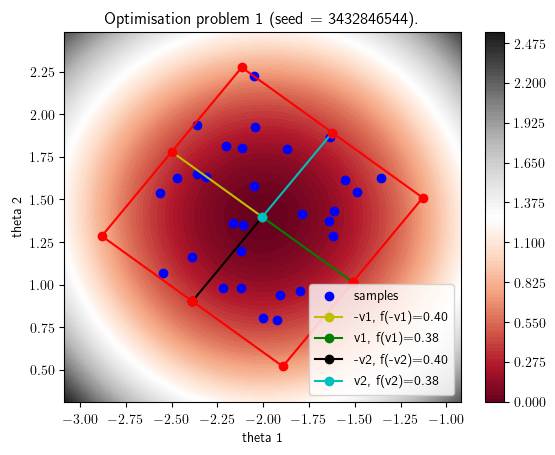
\includegraphics[width=0.48\textwidth]{./Thesis/images/chapter4/ex2D_region_1_bo.png}
    \end{center}
    \caption{Visualisation of the acceptance region in 3 different
      optimisation problems. Each row illustrates a different
      optimisation problem, the left column corresponds to the
      gradient-based approach and the right column to the Bayesian
      optimisation approach. The examples have been chosen to
      illustrate three different cases; in the first case, both
      optimisation schemes lead to similar optimal point and bounding
      box, in the second case the bounding box is similar in shape but
      a little bit shifted to the right relatively to the
      gradient-based approach and in the third case, both the optimal
      point and the bounding box is completely different.}
  \label{fig:ex2_2}
\end{figure}


\begin{figure}[h]
    \begin{center}
      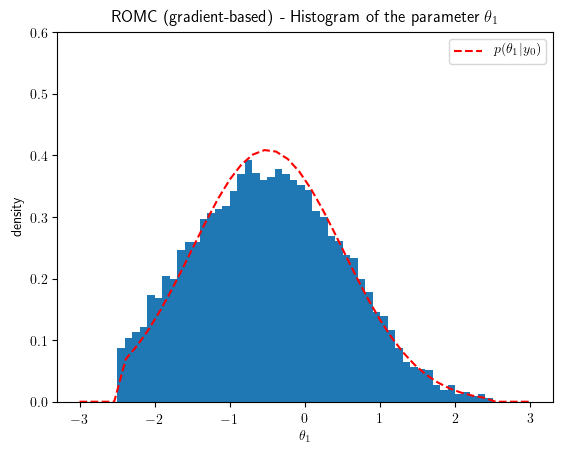
\includegraphics[width=0.48\textwidth]{./Thesis/images/chapter4/ex2D_hist_t1_romc.png}
      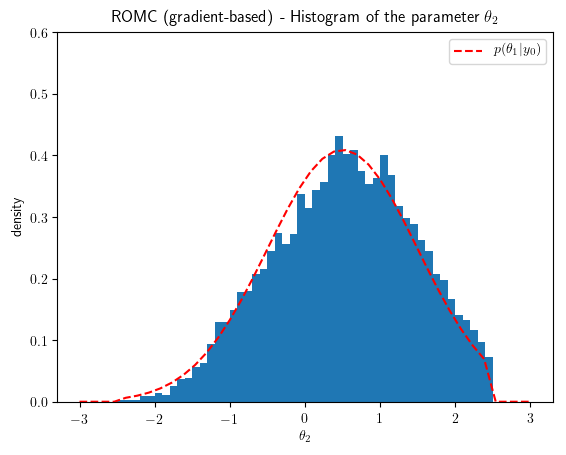
\includegraphics[width=0.48\textwidth]{./Thesis/images/chapter4/ex2D_hist_t2_romc.png}\\
      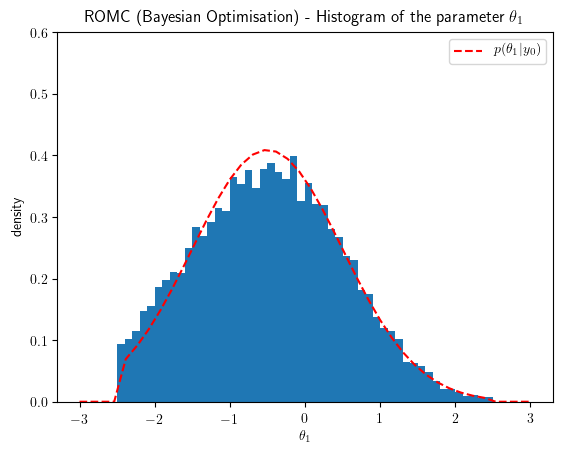
\includegraphics[width=0.48\textwidth]{./Thesis/images/chapter4/ex2D_hist_t1_romc_bo.png}
      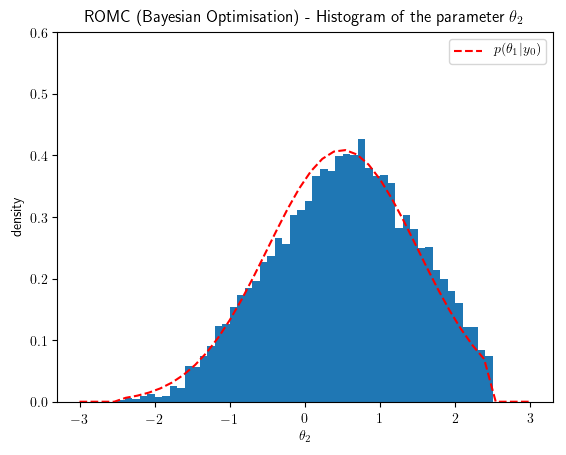
\includegraphics[width=0.48\textwidth]{./Thesis/images/chapter4/ex2D_hist_t2_romc_bo.png}\\
    \end{center}
    \caption{Histogram of the marginal distribution for three
      different inference approaches; (a) in the first row, the
      approximate posterior samples are obtained using Rejection ABC
      sampling (b) in the second row, using ROMC sampling with
      gradient-based approach and (c) in the third row, using ROMC
      sampling with Bayesian optimisation approach. The vertical (red)
      line represents the samples mean $\mu$ and the horizontal
      (black) the standard deviation $\sigma$.}
  \label{fig:ex2_3}
\end{figure}

\begin{figure}[h]
  \begin{center}
      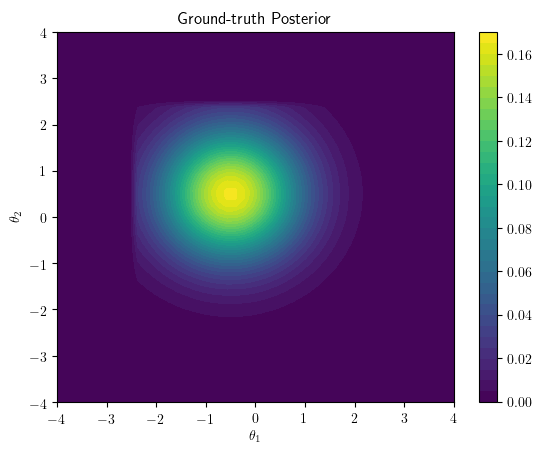
\includegraphics[width=0.5\textwidth]{./Thesis/images/chapter4/ex2D_gt_posterior.png}\\
      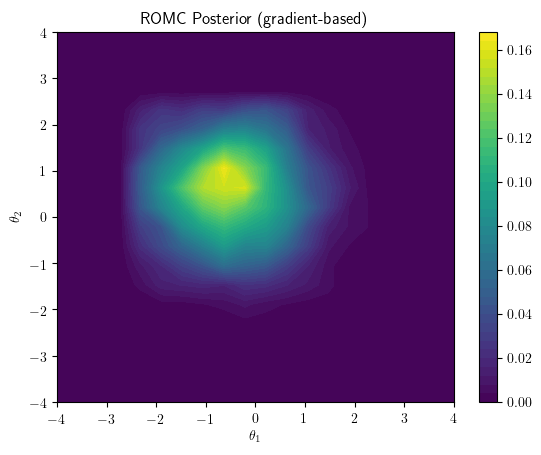
\includegraphics[width=0.48\textwidth]{./Thesis/images/chapter4/ex2D_romc_posterior.png}
      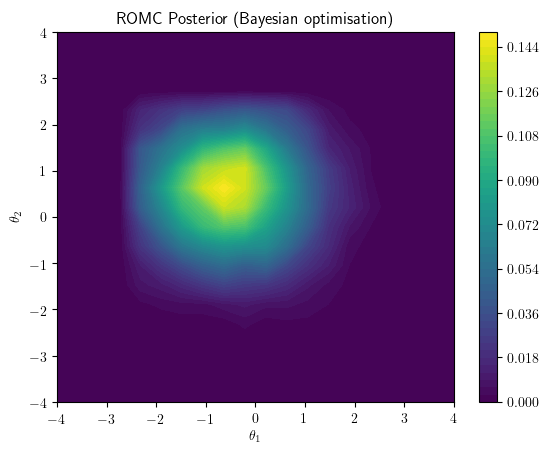
\includegraphics[width=0.48\textwidth]{./Thesis/images/chapter4/ex2D_romc_posterior_bo.png}
    \end{center}
    \caption{(a) First row: Ground-truth posterior approximated
      computationally. (b) ROMC approximate posteriors using
      gradient-based approach (left) and Bayesian optimisation
      approach (right).}
  \label{fig:ex2_4}
\end{figure}

